\documentclass[aspectratio=169]{beamer}

% Minimal theme
\usetheme{default}
\usecolortheme{dove}

% Remove navigation symbols
\setbeamertemplate{navigation symbols}{}
\setbeamertemplate{footline}{%
  \hfill{\large\insertframenumber\,/\,\inserttotalframenumber}\hspace{0.8em}\vspace{0.5em}%
}

% Colors
\definecolor{popblue}{RGB}{52, 101, 164}
\definecolor{sampred}{RGB}{204, 0, 0}
\definecolor{paramgreen}{RGB}{0, 140, 70}
\definecolor{lightbg}{RGB}{245, 245, 250}
\definecolor{warnred}{RGB}{180, 40, 40}
\definecolor{orange1}{RGB}{220, 120, 0}
\definecolor{violet1}{RGB}{120, 50, 160}

\setbeamercolor{frametitle}{fg=popblue}
\setbeamercolor{title}{fg=popblue}

% Packages
\usepackage{pgfplots}
\usepackage{tikz}
\usetikzlibrary{shapes, arrows.meta, positioning, calc, decorations.pathreplacing, patterns}
\pgfplotsset{compat=1.18}
\usepackage{amsmath, amssymb}
\usepackage{array}
\usepackage{fontenc}

\title{Early Notable Models}
\subtitle{ELMo $\cdot$ GPT $\cdot$ BERT $\cdot$ GPT-2 $\cdot$ T5 $\cdot$ GPT-3}
\date{}

\begin{document}

% ============================================================
% TITLE
% ============================================================
\begin{frame}
\titlepage
\end{frame}

% ============================================================
% TIMELINE
% ============================================================
\begin{frame}
\frametitle{The timeline: 2018--2020}

\begin{center}
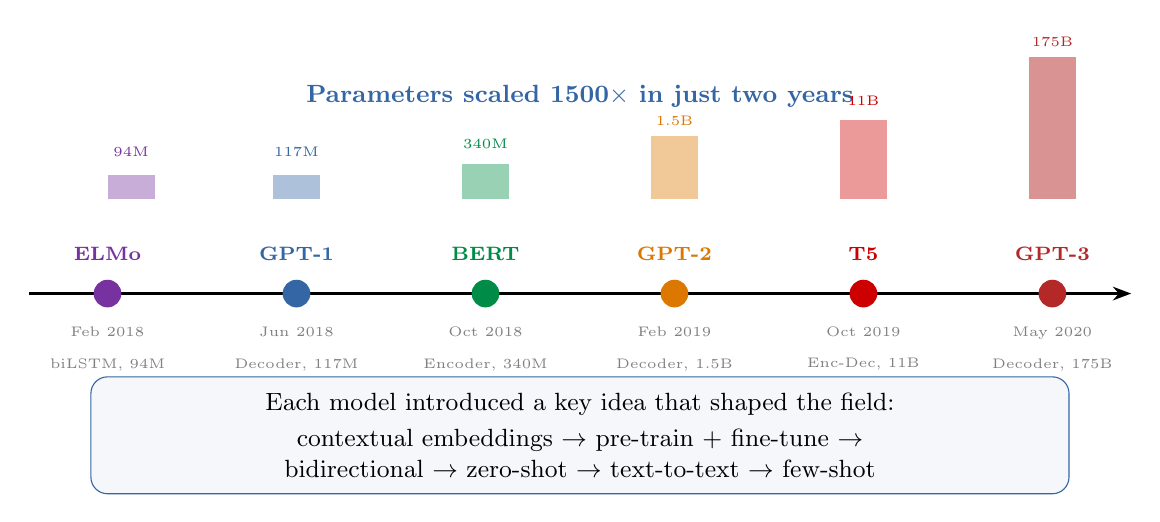
\begin{tikzpicture}
  % Timeline axis
  \draw[thick, -Stealth] (-7, 0) -- (7, 0);

  % ELMo
  \fill[violet1] (-6, 0) circle (5pt);
  \node[font=\scriptsize\bfseries, text=violet1, above] at (-6, 0.3) {ELMo};
  \node[font=\tiny, text=gray, below] at (-6, -0.3) {Feb 2018};
  \node[font=\tiny, text=gray, below] at (-6, -0.7) {biLSTM, 94M};

  % GPT-1
  \fill[popblue] (-3.6, 0) circle (5pt);
  \node[font=\scriptsize\bfseries, text=popblue, above] at (-3.6, 0.3) {GPT-1};
  \node[font=\tiny, text=gray, below] at (-3.6, -0.3) {Jun 2018};
  \node[font=\tiny, text=gray, below] at (-3.6, -0.7) {Decoder, 117M};

  % BERT
  \fill[paramgreen] (-1.2, 0) circle (5pt);
  \node[font=\scriptsize\bfseries, text=paramgreen, above] at (-1.2, 0.3) {BERT};
  \node[font=\tiny, text=gray, below] at (-1.2, -0.3) {Oct 2018};
  \node[font=\tiny, text=gray, below] at (-1.2, -0.7) {Encoder, 340M};

  % GPT-2
  \fill[orange1] (1.2, 0) circle (5pt);
  \node[font=\scriptsize\bfseries, text=orange1, above] at (1.2, 0.3) {GPT-2};
  \node[font=\tiny, text=gray, below] at (1.2, -0.3) {Feb 2019};
  \node[font=\tiny, text=gray, below] at (1.2, -0.7) {Decoder, 1.5B};

  % T5
  \fill[sampred] (3.6, 0) circle (5pt);
  \node[font=\scriptsize\bfseries, text=sampred, above] at (3.6, 0.3) {T5};
  \node[font=\tiny, text=gray, below] at (3.6, -0.3) {Oct 2019};
  \node[font=\tiny, text=gray, below] at (3.6, -0.7) {Enc-Dec, 11B};

  % GPT-3
  \fill[warnred] (6, 0) circle (5pt);
  \node[font=\scriptsize\bfseries, text=warnred, above] at (6, 0.3) {GPT-3};
  \node[font=\tiny, text=gray, below] at (6, -0.3) {May 2020};
  \node[font=\tiny, text=gray, below] at (6, -0.7) {Decoder, 175B};

  % Parameter scaling visual
  \node[font=\small\bfseries, text=popblue] at (0, 2.5) {Parameters scaled 1500$\times$ in just two years};

  % Bars showing parameter counts (log scale visual)
  \fill[violet1!40] (-6, 1.2) rectangle (-5.4, 1.5);
  \fill[popblue!40] (-3.9, 1.2) rectangle (-3.3, 1.5);
  \fill[paramgreen!40] (-1.5, 1.2) rectangle (-0.9, 1.65);
  \fill[orange1!40] (0.9, 1.2) rectangle (1.5, 2);
  \fill[sampred!40] (3.3, 1.2) rectangle (3.9, 2.2);
  \fill[warnred!50] (5.7, 1.2) rectangle (6.3, 3);

  \node[font=\tiny, text=violet1] at (-5.7, 1.8) {94M};
  \node[font=\tiny, text=popblue] at (-3.6, 1.8) {117M};
  \node[font=\tiny, text=paramgreen] at (-1.2, 1.9) {340M};
  \node[font=\tiny, text=orange1] at (1.2, 2.2) {1.5B};
  \node[font=\tiny, text=sampred] at (3.6, 2.45) {11B};
  \node[font=\tiny, text=warnred] at (6, 3.2) {175B};

  % Themes
  \node[draw=popblue, fill=popblue!5, rounded corners=6pt, text width=12cm, align=center, inner sep=6pt, font=\small] at (0, -1.8) {
    Each model introduced a key idea that shaped the field:\\[2pt]
    contextual embeddings $\to$ pre-train + fine-tune $\to$ bidirectional $\to$ zero-shot $\to$ text-to-text $\to$ few-shot
  };
\end{tikzpicture}
\end{center}
\end{frame}

% ============================================================
% ELMo
% ============================================================
\begin{frame}
\frametitle{ELMo --- contextual embeddings (2018)}

\begin{center}
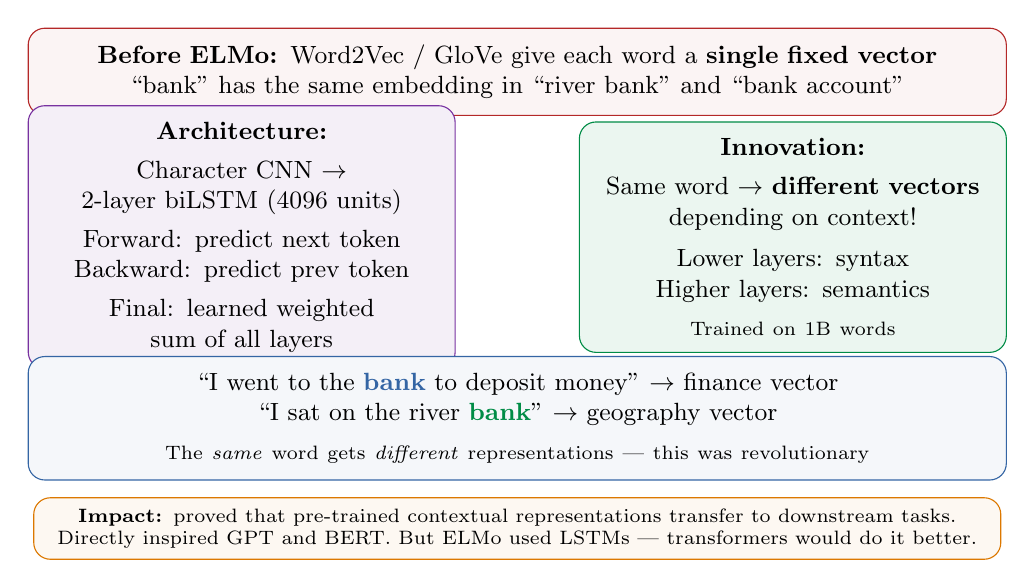
\begin{tikzpicture}
  % The problem
  \node[draw=warnred, fill=warnred!5, rounded corners=6pt, text width=12cm, align=center, inner sep=6pt, font=\small] at (0, 3) {
    \textbf{Before ELMo:} Word2Vec / GloVe give each word a \textbf{single fixed vector}\\
    ``bank'' has the same embedding in ``river bank'' and ``bank account''
  };

  % Architecture
  \node[draw=violet1, fill=violet1!8, rounded corners=6pt, text width=5cm, align=center, inner sep=6pt, font=\small] at (-3.5, 0.9) {
    \textbf{Architecture:}\\[3pt]
    Character CNN $\to$\\2-layer biLSTM (4096 units)\\[3pt]
    Forward: predict next token\\Backward: predict prev token\\[3pt]
    Final: learned weighted sum of all layers
  };

  % The innovation
  \node[draw=paramgreen, fill=paramgreen!8, rounded corners=6pt, text width=5cm, align=center, inner sep=6pt, font=\small] at (3.5, 0.9) {
    \textbf{Innovation:}\\[3pt]
    Same word $\to$ \textbf{different vectors}\\depending on context!\\[4pt]
    Lower layers: syntax\\Higher layers: semantics\\[3pt]
    {\scriptsize Trained on 1B words}
  };

  % Example
  \node[draw=popblue, fill=popblue!5, rounded corners=6pt, text width=12cm, align=center, inner sep=6pt, font=\small] at (0, -1.4) {
    ``I went to the \textbf{\textcolor{popblue}{bank}} to deposit money'' $\to$ finance vector\\
    ``I sat on the river \textbf{\textcolor{paramgreen}{bank}}'' $\to$ geography vector\\[3pt]
    {\scriptsize The \emph{same} word gets \emph{different} representations --- this was revolutionary}
  };

  % Impact
  \node[draw=orange1, fill=orange1!5, rounded corners=6pt, text width=12cm, align=center, inner sep=4pt, font=\scriptsize] at (0, -2.8) {
    \textbf{Impact:} proved that pre-trained contextual representations transfer to downstream tasks.
    Directly inspired GPT and BERT. But ELMo used LSTMs --- transformers would do it better.
  };
\end{tikzpicture}
\end{center}
\end{frame}

% ============================================================
% GPT-1
% ============================================================
\begin{frame}
\frametitle{GPT-1 --- the pre-train + fine-tune paradigm (2018)}

\begin{center}
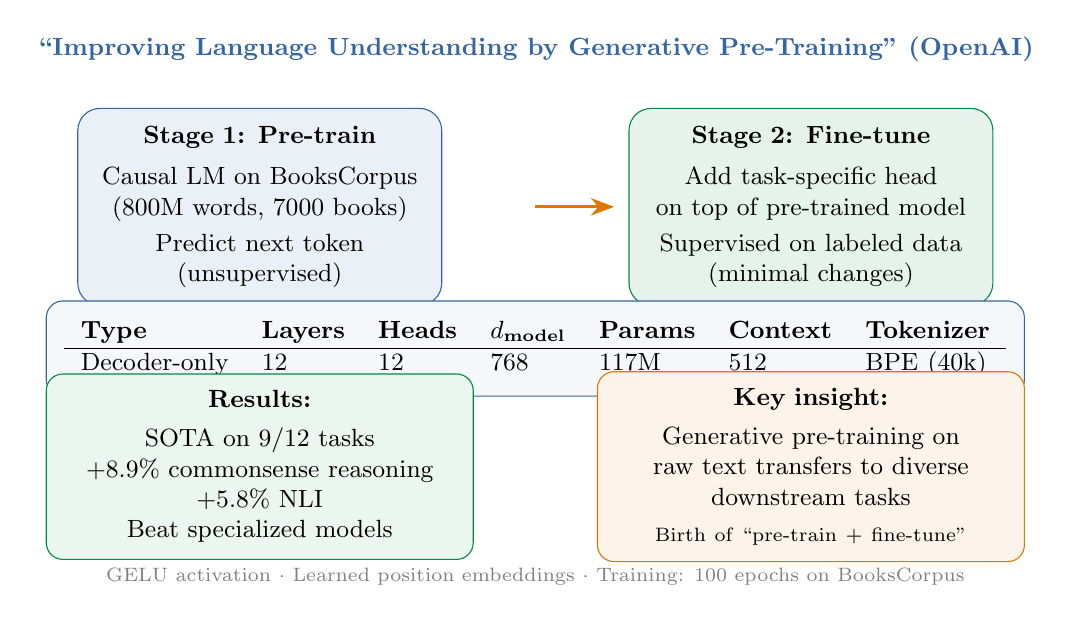
\begin{tikzpicture}
  % Two-stage pipeline
  \node[font=\small\bfseries, text=popblue] at (0, 3.5) {``Improving Language Understanding by Generative Pre-Training'' (OpenAI)};

  % Stage 1
  \node[draw=popblue, fill=popblue!10, rounded corners=8pt, minimum width=4.5cm, minimum height=2.5cm, text width=4.2cm, align=center, inner sep=6pt, font=\small] at (-3.5, 1.5) {
    \textbf{Stage 1: Pre-train}\\[4pt]
    Causal LM on BooksCorpus\\(800M words, 7000 books)\\[2pt]
    Predict next token\\(unsupervised)
  };

  % Stage 2
  \node[draw=paramgreen, fill=paramgreen!10, rounded corners=8pt, minimum width=4.5cm, minimum height=2.5cm, text width=4.2cm, align=center, inner sep=6pt, font=\small] at (3.5, 1.5) {
    \textbf{Stage 2: Fine-tune}\\[4pt]
    Add task-specific head\\on top of pre-trained model\\[2pt]
    Supervised on labeled data\\(minimal changes)
  };

  \draw[-Stealth, very thick, orange1] (0, 1.5) -- (1, 1.5);

  % Architecture
  \node[draw=popblue, fill=popblue!5, rounded corners=6pt, text width=12cm, align=center, inner sep=6pt] at (0, -0.3) {
    {\small
    \begin{tabular}{l l l l l l l}
      \textbf{Type} & \textbf{Layers} & \textbf{Heads} & \textbf{$d_{\text{model}}$} & \textbf{Params} & \textbf{Context} & \textbf{Tokenizer} \\
      \hline
      Decoder-only & 12 & 12 & 768 & 117M & 512 & BPE (40k)
    \end{tabular}
    }
  };

  % Results
  \node[draw=paramgreen, fill=paramgreen!8, rounded corners=6pt, text width=5cm, align=center, inner sep=6pt, font=\small] at (-3.5, -1.8) {
    \textbf{Results:}\\[3pt]
    SOTA on 9/12 tasks\\+8.9\% commonsense reasoning\\+5.8\% NLI\\Beat specialized models
  };

  % Key insight
  \node[draw=orange1, fill=orange1!8, rounded corners=6pt, text width=5cm, align=center, inner sep=6pt, font=\small] at (3.5, -1.8) {
    \textbf{Key insight:}\\[3pt]
    Generative pre-training on\\raw text transfers to diverse\\downstream tasks\\[2pt]
    {\scriptsize Birth of ``pre-train + fine-tune''}
  };

  % Bottom
  \node[font=\scriptsize, text=gray] at (0, -3.2) {
    GELU activation $\cdot$ Learned position embeddings $\cdot$ Training: 100 epochs on BooksCorpus
  };
\end{tikzpicture}
\end{center}
\end{frame}

% ============================================================
% BERT: THE BREAKTHROUGH
% ============================================================
\begin{frame}
\frametitle{BERT --- bidirectional is better (2018)}

\begin{center}
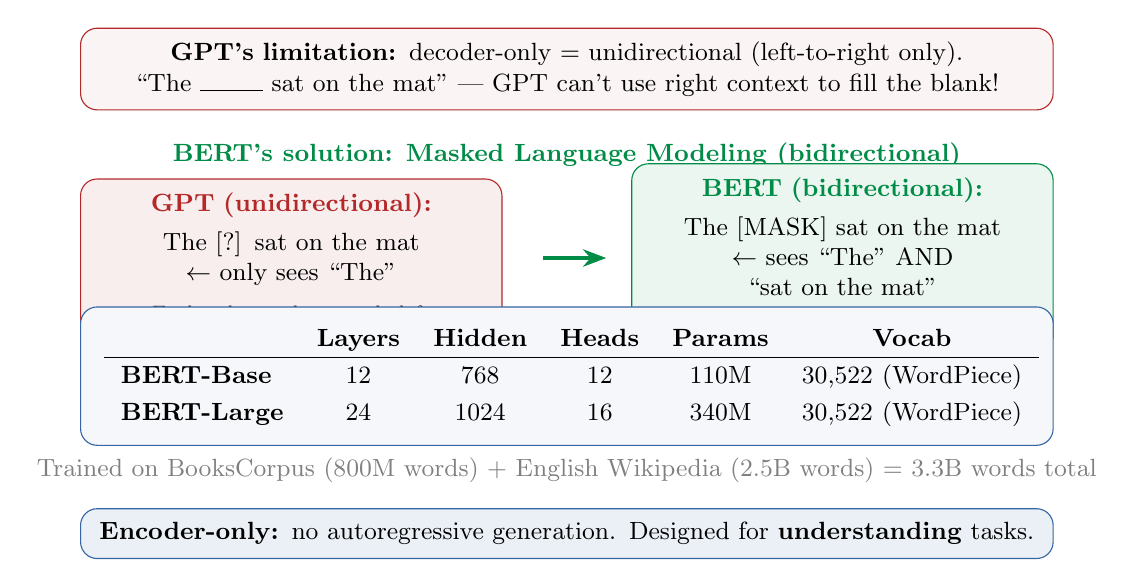
\begin{tikzpicture}
  % The limitation of GPT
  \node[draw=warnred, fill=warnred!5, rounded corners=6pt, text width=12cm, align=center, inner sep=5pt, font=\small] at (0, 3) {
    \textbf{GPT's limitation:} decoder-only = unidirectional (left-to-right only).\\
    ``The \rule{0.8cm}{0.4pt} sat on the mat'' --- GPT can't use right context to fill the blank!
  };

  % BERT's solution
  \node[font=\small\bfseries, text=paramgreen] at (0, 1.9) {BERT's solution: Masked Language Modeling (bidirectional)};

  % Unidirectional vs bidirectional
  \node[draw=warnred, fill=warnred!8, rounded corners=6pt, text width=5cm, align=center, inner sep=5pt, font=\small] at (-3.5, 0.6) {
    \textbf{\textcolor{warnred}{GPT (unidirectional):}}\\[3pt]
    The [?] sat on the mat\\$\leftarrow$ only sees ``The''\\[3pt]
    {\scriptsize Each token only attends left}
  };

  \node[draw=paramgreen, fill=paramgreen!8, rounded corners=6pt, text width=5cm, align=center, inner sep=5pt, font=\small] at (3.5, 0.6) {
    \textbf{\textcolor{paramgreen}{BERT (bidirectional):}}\\[3pt]
    The [MASK] sat on the mat\\$\leftarrow$ sees ``The'' AND ``sat on the mat''\\[3pt]
    {\scriptsize Each token attends to ALL positions}
  };

  \draw[-Stealth, very thick, paramgreen] (-0.3, 0.6) -- (0.5, 0.6);

  % Architecture table
  \node[draw=popblue, fill=popblue!5, rounded corners=6pt, text width=12cm, align=center, inner sep=5pt] at (0, -0.9) {
    {\small
    \renewcommand{\arraystretch}{1.2}
    \begin{tabular}{l c c c c c}
      & \textbf{Layers} & \textbf{Hidden} & \textbf{Heads} & \textbf{Params} & \textbf{Vocab} \\
      \hline
      \textbf{BERT-Base} & 12 & 768 & 12 & 110M & 30,522 (WordPiece) \\
      \textbf{BERT-Large} & 24 & 1024 & 16 & 340M & 30,522 (WordPiece) \\
    \end{tabular}
    }
  };

  % Training data
  \node[font=\small, text=gray] at (0, -2.1) {
    Trained on BooksCorpus (800M words) + English Wikipedia (2.5B words) = 3.3B words total
  };

  % Bottom
  \node[draw=popblue, fill=popblue!10, rounded corners=6pt, text width=12cm, align=center, inner sep=5pt, font=\small] at (0, -2.9) {
    \textbf{Encoder-only:} no autoregressive generation. Designed for \textbf{understanding} tasks.
  };
\end{tikzpicture}
\end{center}
\end{frame}

% ============================================================
% BERT: INPUT FORMAT
% ============================================================
\begin{frame}
\frametitle{BERT --- input format and special tokens}

\begin{center}
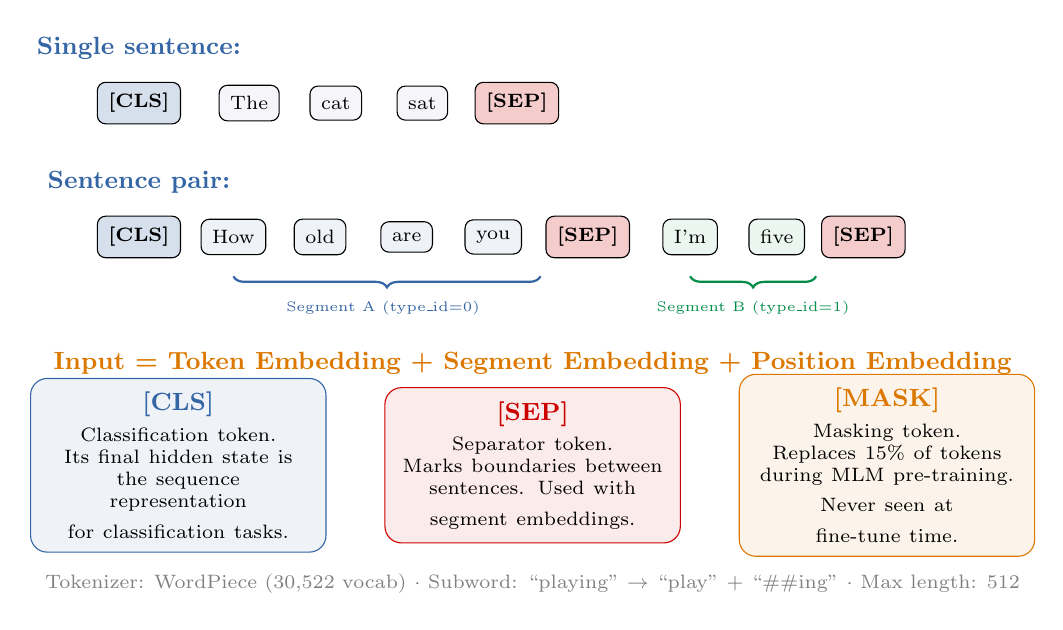
\begin{tikzpicture}
  % Single sentence
  \node[font=\small\bfseries, text=popblue] at (-5, 3.5) {Single sentence:};

  \node[draw, rounded corners=3pt, fill=popblue!20, inner sep=4pt, font=\scriptsize\bfseries] at (-5, 2.8) {[CLS]};
  \node[draw, rounded corners=3pt, fill=lightbg, inner sep=4pt, font=\scriptsize] at (-3.6, 2.8) {The};
  \node[draw, rounded corners=3pt, fill=lightbg, inner sep=4pt, font=\scriptsize] at (-2.5, 2.8) {cat};
  \node[draw, rounded corners=3pt, fill=lightbg, inner sep=4pt, font=\scriptsize] at (-1.4, 2.8) {sat};
  \node[draw, rounded corners=3pt, fill=sampred!20, inner sep=4pt, font=\scriptsize\bfseries] at (-0.2, 2.8) {[SEP]};

  % Sentence pair
  \node[font=\small\bfseries, text=popblue] at (-5, 1.8) {Sentence pair:};

  \node[draw, rounded corners=3pt, fill=popblue!20, inner sep=4pt, font=\scriptsize\bfseries] at (-5, 1.1) {[CLS]};
  \node[draw, rounded corners=3pt, fill=popblue!8, inner sep=4pt, font=\scriptsize] at (-3.8, 1.1) {How};
  \node[draw, rounded corners=3pt, fill=popblue!8, inner sep=4pt, font=\scriptsize] at (-2.7, 1.1) {old};
  \node[draw, rounded corners=3pt, fill=popblue!8, inner sep=4pt, font=\scriptsize] at (-1.6, 1.1) {are};
  \node[draw, rounded corners=3pt, fill=popblue!8, inner sep=4pt, font=\scriptsize] at (-0.5, 1.1) {you};
  \node[draw, rounded corners=3pt, fill=sampred!20, inner sep=4pt, font=\scriptsize\bfseries] at (0.7, 1.1) {[SEP]};
  \node[draw, rounded corners=3pt, fill=paramgreen!8, inner sep=4pt, font=\scriptsize] at (2, 1.1) {I'm};
  \node[draw, rounded corners=3pt, fill=paramgreen!8, inner sep=4pt, font=\scriptsize] at (3.1, 1.1) {five};
  \node[draw, rounded corners=3pt, fill=sampred!20, inner sep=4pt, font=\scriptsize\bfseries] at (4.2, 1.1) {[SEP]};

  % Segment labels
  \draw[decorate, decoration={brace, amplitude=4pt, mirror}, thick, popblue] (-3.8, 0.6) -- (0.1, 0.6);
  \node[font=\tiny, text=popblue] at (-1.9, 0.2) {Segment A (type\_id=0)};
  \draw[decorate, decoration={brace, amplitude=4pt, mirror}, thick, paramgreen] (2, 0.6) -- (3.6, 0.6);
  \node[font=\tiny, text=paramgreen] at (2.8, 0.2) {Segment B (type\_id=1)};

  % Three embeddings
  \node[font=\small\bfseries, text=orange1] at (0, -0.5) {Input = Token Embedding + Segment Embedding + Position Embedding};

  % Special tokens explained
  \node[draw=popblue, fill=popblue!8, rounded corners=6pt, text width=3.4cm, align=center, inner sep=5pt, font=\small] at (-4.5, -1.8) {
    \textbf{\textcolor{popblue}{[CLS]}}\\[3pt]
    {\scriptsize Classification token.\\Its final hidden state is\\the sequence representation\\for classification tasks.}
  };

  \node[draw=sampred, fill=sampred!8, rounded corners=6pt, text width=3.4cm, align=center, inner sep=5pt, font=\small] at (0, -1.8) {
    \textbf{\textcolor{sampred}{[SEP]}}\\[3pt]
    {\scriptsize Separator token.\\Marks boundaries between\\sentences. Used with\\segment embeddings.}
  };

  \node[draw=orange1, fill=orange1!8, rounded corners=6pt, text width=3.4cm, align=center, inner sep=5pt, font=\small] at (4.5, -1.8) {
    \textbf{\textcolor{orange1}{[MASK]}}\\[3pt]
    {\scriptsize Masking token.\\Replaces 15\% of tokens\\during MLM pre-training.\\Never seen at fine-tune time.}
  };

  % WordPiece
  \node[font=\scriptsize, text=gray] at (0, -3.3) {
    Tokenizer: WordPiece (30,522 vocab) $\cdot$ Subword: ``playing'' $\to$ ``play'' + ``\#\#ing'' $\cdot$ Max length: 512
  };
\end{tikzpicture}
\end{center}
\end{frame}

% ============================================================
% BERT: TRAINING OBJECTIVES
% ============================================================
\begin{frame}
\frametitle{BERT --- pre-training objectives}

\begin{center}
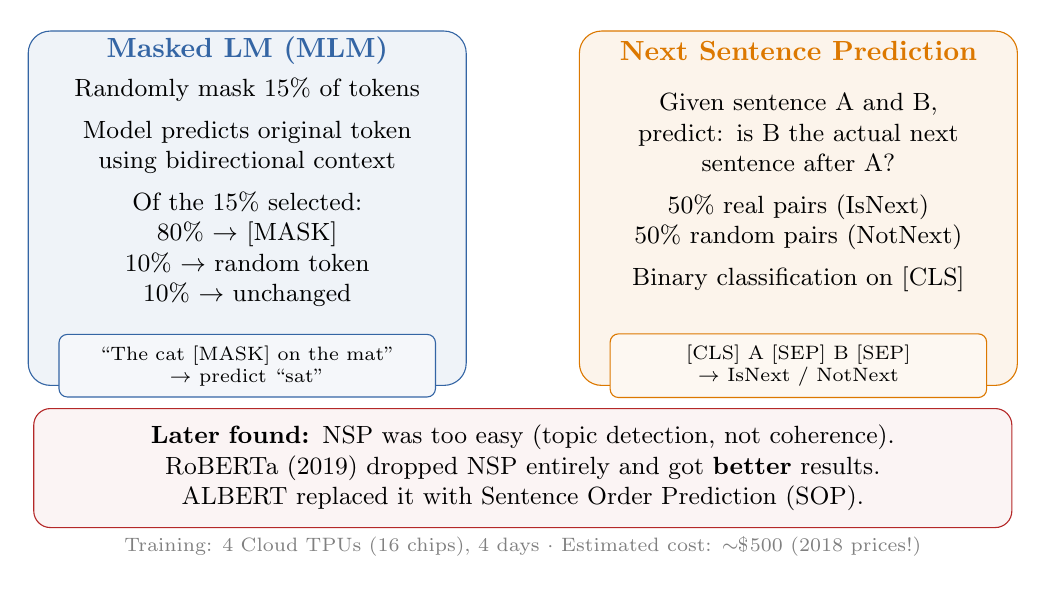
\begin{tikzpicture}
  % MLM
  \node[draw=popblue, fill=popblue!8, rounded corners=8pt, minimum width=5.5cm, minimum height=4.5cm, text width=5cm, align=center, inner sep=8pt] at (-3.5, 1) {};
  \node[font=\normalsize\bfseries, text=popblue] at (-3.5, 3) {Masked LM (MLM)};

  \node[font=\small, text width=4.5cm, align=center] at (-3.5, 1.2) {
    Randomly mask 15\% of tokens\\[4pt]
    Model predicts original token\\using bidirectional context\\[4pt]
    Of the 15\% selected:\\80\% $\to$ [MASK]\\10\% $\to$ random token\\10\% $\to$ unchanged
  };

  \node[draw=popblue, fill=popblue!5, rounded corners=3pt, font=\scriptsize, text width=4.5cm, align=center, inner sep=4pt] at (-3.5, -1) {
    ``The cat [MASK] on the mat''\\$\to$ predict ``sat''
  };

  % NSP
  \node[draw=orange1, fill=orange1!8, rounded corners=8pt, minimum width=5.5cm, minimum height=4.5cm, text width=5cm, align=center, inner sep=8pt] at (3.5, 1) {};
  \node[font=\normalsize\bfseries, text=orange1] at (3.5, 3) {Next Sentence Prediction};

  \node[font=\small, text width=4.5cm, align=center] at (3.5, 1.2) {
    Given sentence A and B,\\predict: is B the actual next\\sentence after A?\\[4pt]
    50\% real pairs (IsNext)\\50\% random pairs (NotNext)\\[4pt]
    Binary classification on [CLS]
  };

  \node[draw=orange1, fill=orange1!5, rounded corners=3pt, font=\scriptsize, text width=4.5cm, align=center, inner sep=4pt] at (3.5, -1) {
    [CLS] A [SEP] B [SEP]\\$\to$ IsNext / NotNext
  };

  % Note about NSP
  \node[draw=warnred, fill=warnred!5, rounded corners=6pt, text width=12cm, align=center, inner sep=6pt, font=\small] at (0, -2.3) {
    \textbf{Later found:} NSP was too easy (topic detection, not coherence).\\
    RoBERTa (2019) dropped NSP entirely and got \textbf{better} results.\\
    ALBERT replaced it with Sentence Order Prediction (SOP).
  };

  % Training cost
  \node[font=\scriptsize, text=gray] at (0, -3.3) {
    Training: 4 Cloud TPUs (16 chips), 4 days $\cdot$ Estimated cost: $\sim$\$500 (2018 prices!)
  };
\end{tikzpicture}
\end{center}
\end{frame}

% ============================================================
% BERT: RESULTS
% ============================================================
\begin{frame}
\frametitle{BERT --- why everyone lost their minds}

\begin{center}
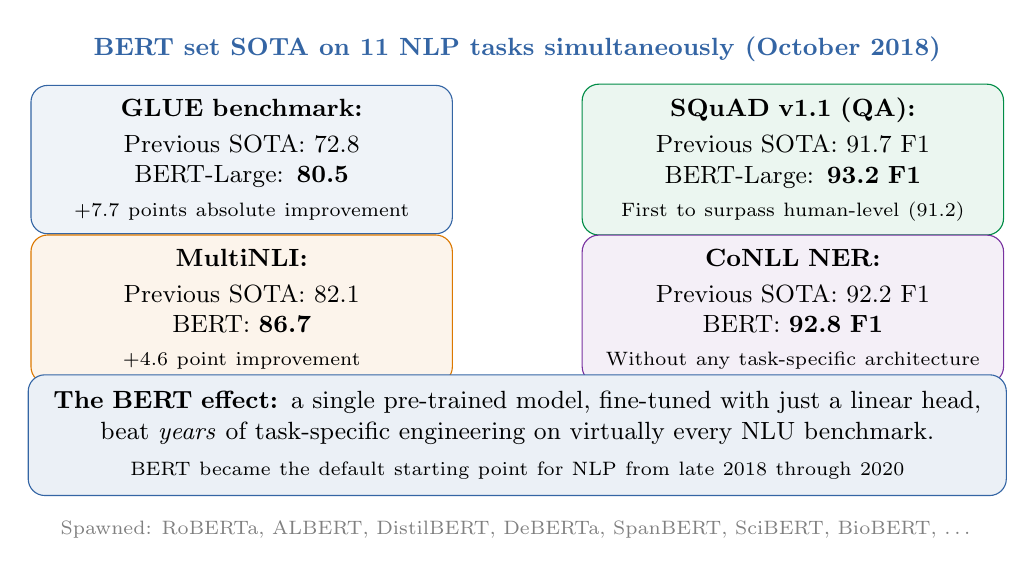
\begin{tikzpicture}
  \node[font=\small\bfseries, text=popblue] at (0, 3.2) {BERT set SOTA on \textbf{11 NLP tasks simultaneously} (October 2018)};

  % GLUE
  \node[draw=popblue, fill=popblue!8, rounded corners=6pt, text width=5cm, align=center, inner sep=5pt, font=\small] at (-3.5, 1.8) {
    \textbf{GLUE benchmark:}\\[2pt]
    Previous SOTA: 72.8\\BERT-Large: \textbf{80.5}\\[1pt]
    {\scriptsize +7.7 points absolute improvement}
  };

  % SQuAD
  \node[draw=paramgreen, fill=paramgreen!8, rounded corners=6pt, text width=5cm, align=center, inner sep=5pt, font=\small] at (3.5, 1.8) {
    \textbf{SQuAD v1.1 (QA):}\\[2pt]
    Previous SOTA: 91.7 F1\\BERT-Large: \textbf{93.2 F1}\\[1pt]
    {\scriptsize First to surpass human-level (91.2)}
  };

  % NLI
  \node[draw=orange1, fill=orange1!8, rounded corners=6pt, text width=5cm, align=center, inner sep=5pt, font=\small] at (-3.5, -0.1) {
    \textbf{MultiNLI:}\\[2pt]
    Previous SOTA: 82.1\\BERT: \textbf{86.7}\\[1pt]
    {\scriptsize +4.6 point improvement}
  };

  % NER
  \node[draw=violet1, fill=violet1!8, rounded corners=6pt, text width=5cm, align=center, inner sep=5pt, font=\small] at (3.5, -0.1) {
    \textbf{CoNLL NER:}\\[2pt]
    Previous SOTA: 92.2 F1\\BERT: \textbf{92.8 F1}\\[1pt]
    {\scriptsize Without any task-specific architecture}
  };

  % Impact
  \node[draw=popblue, fill=popblue!10, rounded corners=6pt, text width=12cm, align=center, inner sep=6pt, font=\small] at (0, -1.7) {
    \textbf{The BERT effect:} a single pre-trained model, fine-tuned with just a linear head,\\
    beat \emph{years} of task-specific engineering on virtually every NLU benchmark.\\[2pt]
    {\scriptsize BERT became the default starting point for NLP from late 2018 through 2020}
  };

  % Spawned
  \node[font=\scriptsize, text=gray] at (0, -2.9) {
    Spawned: RoBERTa, ALBERT, DistilBERT, DeBERTa, SpanBERT, SciBERT, BioBERT, \ldots
  };
\end{tikzpicture}
\end{center}
\end{frame}

% ============================================================
% THREE ARCHITECTURES
% ============================================================
\begin{frame}
\frametitle{Three architectures, three strengths}

\begin{center}
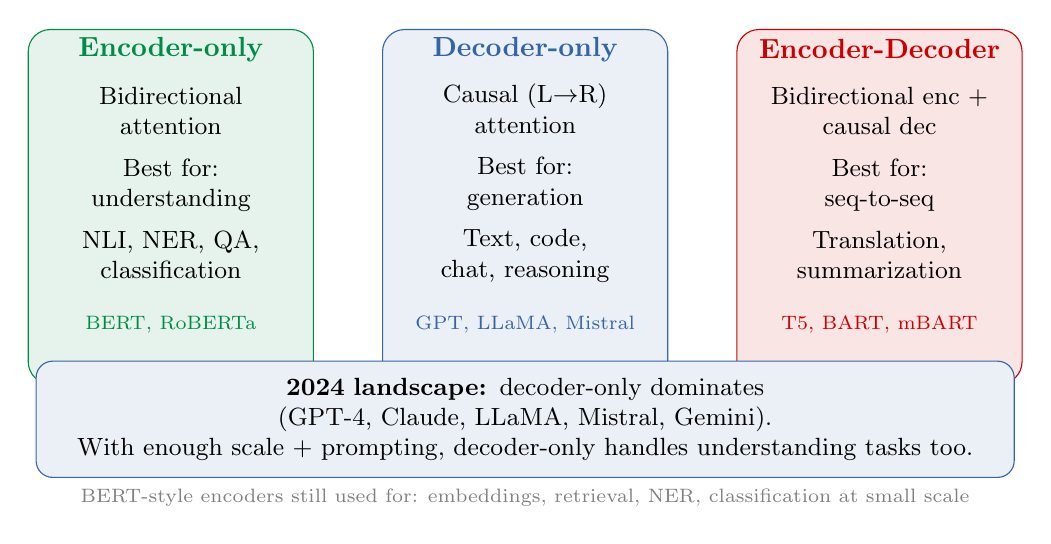
\begin{tikzpicture}
  % Encoder-only
  \node[draw=paramgreen, fill=paramgreen!10, rounded corners=8pt, minimum width=3.5cm, minimum height=4.5cm, text width=3.2cm, align=center, inner sep=6pt] at (-4.5, 0.5) {};
  \node[font=\normalsize\bfseries, text=paramgreen] at (-4.5, 2.5) {Encoder-only};

  \node[font=\small, text width=3cm, align=center] at (-4.5, 0.8) {
    Bidirectional\\attention\\[4pt]
    Best for:\\understanding\\[4pt]
    NLI, NER, QA,\\classification
  };
  \node[font=\scriptsize, text=paramgreen] at (-4.5, -1) {BERT, RoBERTa};

  % Decoder-only
  \node[draw=popblue, fill=popblue!10, rounded corners=8pt, minimum width=3.5cm, minimum height=4.5cm, text width=3.2cm, align=center, inner sep=6pt] at (0, 0.5) {};
  \node[font=\normalsize\bfseries, text=popblue] at (0, 2.5) {Decoder-only};

  \node[font=\small, text width=3cm, align=center] at (0, 0.8) {
    Causal (L$\to$R)\\attention\\[4pt]
    Best for:\\generation\\[4pt]
    Text, code,\\chat, reasoning
  };
  \node[font=\scriptsize, text=popblue] at (0, -1) {GPT, LLaMA, Mistral};

  % Encoder-decoder
  \node[draw=sampred, fill=sampred!10, rounded corners=8pt, minimum width=3.5cm, minimum height=4.5cm, text width=3.2cm, align=center, inner sep=6pt] at (4.5, 0.5) {};
  \node[font=\normalsize\bfseries, text=sampred] at (4.5, 2.5) {Encoder-Decoder};

  \node[font=\small, text width=3cm, align=center] at (4.5, 0.8) {
    Bidirectional enc +\\causal dec\\[4pt]
    Best for:\\seq-to-seq\\[4pt]
    Translation,\\summarization
  };
  \node[font=\scriptsize, text=sampred] at (4.5, -1) {T5, BART, mBART};

  % Modern dominance
  \node[draw=popblue, fill=popblue!10, rounded corners=6pt, text width=12cm, align=center, inner sep=6pt, font=\small] at (0, -2.2) {
    \textbf{2024 landscape:} decoder-only dominates (GPT-4, Claude, LLaMA, Mistral, Gemini).\\
    With enough scale + prompting, decoder-only handles understanding tasks too.
  };

  \node[font=\scriptsize, text=gray] at (0, -3.2) {
    BERT-style encoders still used for: embeddings, retrieval, NER, classification at small scale
  };
\end{tikzpicture}
\end{center}
\end{frame}

% ============================================================
% GPT-2
% ============================================================
\begin{frame}
\frametitle{GPT-2 --- scaling up, zero-shot emerges (2019)}

\begin{center}
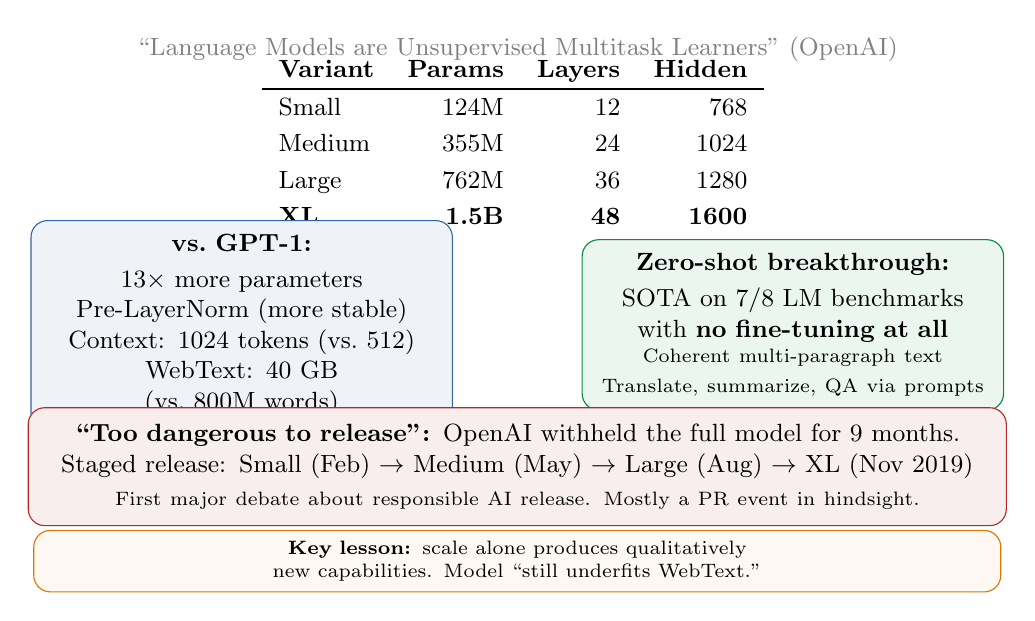
\begin{tikzpicture}
  % Title
  \node[font=\small, text=gray] at (0, 3.3) {``Language Models are Unsupervised Multitask Learners'' (OpenAI)};

  % Size table
  \renewcommand{\arraystretch}{1.2}
  \node at (0, 2.1) {
    {\small
    \begin{tabular}{l r r r}
      \textbf{Variant} & \textbf{Params} & \textbf{Layers} & \textbf{Hidden} \\
      \hline
      Small & 124M & 12 & 768 \\
      Medium & 355M & 24 & 1024 \\
      Large & 762M & 36 & 1280 \\
      \textbf{XL} & \textbf{1.5B} & \textbf{48} & \textbf{1600} \\
    \end{tabular}
    }
  };

  % Key changes from GPT-1
  \node[draw=popblue, fill=popblue!8, rounded corners=6pt, text width=5cm, align=center, inner sep=5pt, font=\small] at (-3.5, -0.2) {
    \textbf{vs.\ GPT-1:}\\[2pt]
    13$\times$ more parameters\\Pre-LayerNorm (more stable)\\Context: 1024 tokens (vs.\ 512)\\WebText: 40 GB (vs.\ 800M words)
  };

  % Zero-shot
  \node[draw=paramgreen, fill=paramgreen!8, rounded corners=6pt, text width=5cm, align=center, inner sep=5pt, font=\small] at (3.5, -0.2) {
    \textbf{Zero-shot breakthrough:}\\[2pt]
    SOTA on 7/8 LM benchmarks\\with \textbf{no fine-tuning at all}\\[1pt]
    {\scriptsize Coherent multi-paragraph text\\Translate, summarize, QA via prompts}
  };

  % "Too dangerous to release"
  \node[draw=warnred, fill=warnred!8, rounded corners=6pt, text width=12cm, align=center, inner sep=6pt, font=\small] at (0, -2) {
    \textbf{``Too dangerous to release'':} OpenAI withheld the full model for 9 months.\\
    Staged release: Small (Feb) $\to$ Medium (May) $\to$ Large (Aug) $\to$ XL (Nov 2019)\\[1pt]
    {\scriptsize First major debate about responsible AI release. Mostly a PR event in hindsight.}
  };

  % Key lesson
  \node[draw=orange1, fill=orange1!5, rounded corners=6pt, text width=12cm, align=center, inner sep=4pt, font=\scriptsize] at (0, -3.2) {
    \textbf{Key lesson:} scale alone produces qualitatively new capabilities. Model ``still underfits WebText.''
  };
\end{tikzpicture}
\end{center}
\end{frame}

% ============================================================
% T5: TEXT-TO-TEXT
% ============================================================
\begin{frame}
\frametitle{T5 --- everything is text-to-text (2019)}

\begin{center}
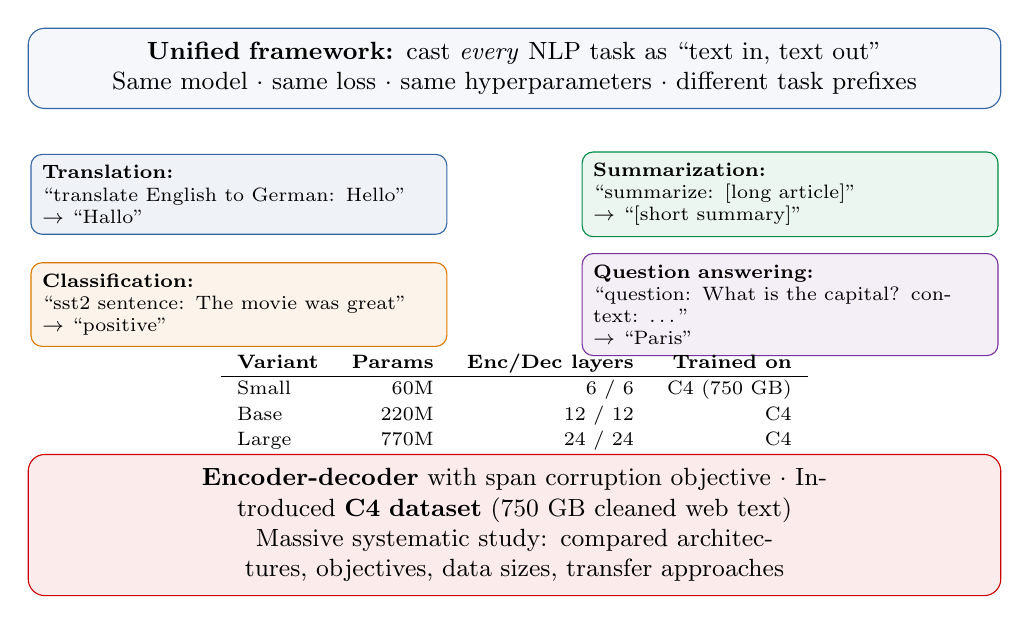
\begin{tikzpicture}
  % The framework
  \node[draw=popblue, fill=popblue!5, rounded corners=6pt, text width=12cm, align=center, inner sep=5pt, font=\small] at (0, 3) {
    \textbf{Unified framework:} cast \emph{every} NLP task as ``text in, text out''\\
    Same model $\cdot$ same loss $\cdot$ same hyperparameters $\cdot$ different task prefixes
  };

  % Task examples
  \node[draw=popblue, fill=popblue!8, rounded corners=4pt, text width=5cm, align=left, inner sep=4pt, font=\scriptsize] at (-3.5, 1.4) {
    \textbf{Translation:}\\
    ``translate English to German: Hello''\\$\to$ ``Hallo''
  };
  \node[draw=paramgreen, fill=paramgreen!8, rounded corners=4pt, text width=5cm, align=left, inner sep=4pt, font=\scriptsize] at (3.5, 1.4) {
    \textbf{Summarization:}\\
    ``summarize: [long article]''\\$\to$ ``[short summary]''
  };
  \node[draw=orange1, fill=orange1!8, rounded corners=4pt, text width=5cm, align=left, inner sep=4pt, font=\scriptsize] at (-3.5, 0) {
    \textbf{Classification:}\\
    ``sst2 sentence: The movie was great''\\$\to$ ``positive''
  };
  \node[draw=violet1, fill=violet1!8, rounded corners=4pt, text width=5cm, align=left, inner sep=4pt, font=\scriptsize] at (3.5, 0) {
    \textbf{Question answering:}\\
    ``question: What is the capital? context: \ldots''\\$\to$ ``Paris''
  };

  % Architecture
  \node at (0, -1.4) {
    {\scriptsize
    \renewcommand{\arraystretch}{1.15}
    \begin{tabular}{l r r r}
      \textbf{Variant} & \textbf{Params} & \textbf{Enc/Dec layers} & \textbf{Trained on} \\
      \hline
      Small & 60M & 6 / 6 & C4 (750 GB) \\
      Base & 220M & 12 / 12 & C4 \\
      Large & 770M & 24 / 24 & C4 \\
      \textbf{11B} & \textbf{11B} & \textbf{24 / 24} & C4 \\
    \end{tabular}
    }
  };

  % Key contributions
  \node[draw=sampred, fill=sampred!8, rounded corners=6pt, text width=12cm, align=center, inner sep=5pt, font=\small] at (0, -2.8) {
    \textbf{Encoder-decoder} with span corruption objective $\cdot$ Introduced \textbf{C4 dataset} (750 GB cleaned web text)\\
    Massive systematic study: compared architectures, objectives, data sizes, transfer approaches
  };
\end{tikzpicture}
\end{center}
\end{frame}

% ============================================================
% T5: THE SYSTEMATIC STUDY
% ============================================================
\begin{frame}
\frametitle{T5 --- the definitive transfer learning study}

\begin{center}
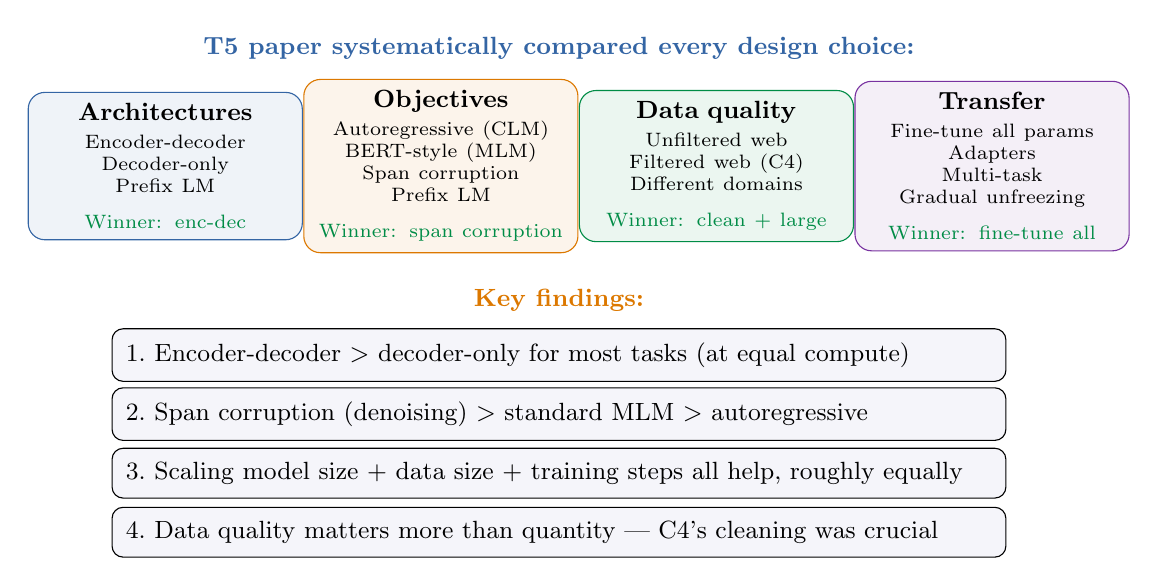
\begin{tikzpicture}
  \node[font=\small\bfseries, text=popblue] at (0, 3.3) {T5 paper systematically compared every design choice:};

  % Architectures
  \node[draw=popblue, fill=popblue!8, rounded corners=6pt, text width=3.2cm, align=center, inner sep=4pt, font=\small] at (-5, 1.8) {
    \textbf{Architectures}\\[2pt]
    {\scriptsize Encoder-decoder\\Decoder-only\\Prefix LM\\[2pt]
    \textcolor{paramgreen}{Winner: enc-dec}}
  };

  % Pre-training objectives
  \node[draw=orange1, fill=orange1!8, rounded corners=6pt, text width=3.2cm, align=center, inner sep=4pt, font=\small] at (-1.5, 1.8) {
    \textbf{Objectives}\\[2pt]
    {\scriptsize Autoregressive (CLM)\\BERT-style (MLM)\\Span corruption\\Prefix LM\\[2pt]
    \textcolor{paramgreen}{Winner: span corruption}}
  };

  % Data
  \node[draw=paramgreen, fill=paramgreen!8, rounded corners=6pt, text width=3.2cm, align=center, inner sep=4pt, font=\small] at (2, 1.8) {
    \textbf{Data quality}\\[2pt]
    {\scriptsize Unfiltered web\\Filtered web (C4)\\Different domains\\[2pt]
    \textcolor{paramgreen}{Winner: clean + large}}
  };

  % Transfer
  \node[draw=violet1, fill=violet1!8, rounded corners=6pt, text width=3.2cm, align=center, inner sep=4pt, font=\small] at (5.5, 1.8) {
    \textbf{Transfer}\\[2pt]
    {\scriptsize Fine-tune all params\\Adapters\\Multi-task\\Gradual unfreezing\\[2pt]
    \textcolor{paramgreen}{Winner: fine-tune all}}
  };

  % Key findings
  \node[font=\small\bfseries, text=orange1] at (0, 0.1) {Key findings:};

  \node[draw, rounded corners=4pt, fill=lightbg, text width=11cm, align=left, inner sep=5pt, font=\small] at (0, -0.6) {
    1.\ Encoder-decoder $>$ decoder-only for most tasks (at equal compute)
  };
  \node[draw, rounded corners=4pt, fill=lightbg, text width=11cm, align=left, inner sep=5pt, font=\small] at (0, -1.35) {
    2.\ Span corruption (denoising) $>$ standard MLM $>$ autoregressive
  };
  \node[draw, rounded corners=4pt, fill=lightbg, text width=11cm, align=left, inner sep=5pt, font=\small] at (0, -2.1) {
    3.\ Scaling model size + data size + training steps all help, roughly equally
  };
  \node[draw, rounded corners=4pt, fill=lightbg, text width=11cm, align=left, inner sep=5pt, font=\small] at (0, -2.85) {
    4.\ Data quality matters more than quantity --- C4's cleaning was crucial
  };
\end{tikzpicture}
\end{center}
\end{frame}

% ============================================================
% GPT-3: THE LEAP
% ============================================================
\begin{frame}
\frametitle{GPT-3 --- the leap to 175B (2020)}

\begin{center}
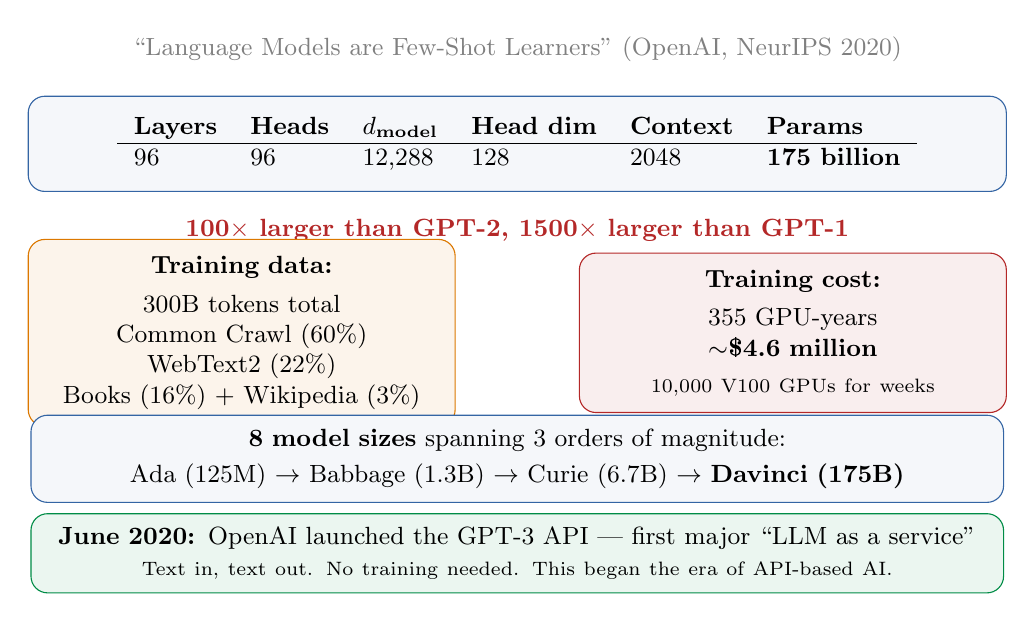
\begin{tikzpicture}
  % Title
  \node[font=\small, text=gray] at (0, 3.5) {``Language Models are Few-Shot Learners'' (OpenAI, NeurIPS 2020)};

  % Architecture
  \node[draw=popblue, fill=popblue!5, rounded corners=6pt, text width=12cm, align=center, inner sep=6pt] at (0, 2.3) {
    {\small
    \begin{tabular}{l l l l l l}
      \textbf{Layers} & \textbf{Heads} & \textbf{$d_{\text{model}}$} & \textbf{Head dim} & \textbf{Context} & \textbf{Params} \\
      \hline
      96 & 96 & 12,288 & 128 & 2048 & \textbf{175 billion}
    \end{tabular}
    }
  };

  % Scale comparison
  \node[font=\small\bfseries, text=warnred] at (0, 1.2) {100$\times$ larger than GPT-2, 1500$\times$ larger than GPT-1};

  % Training data
  \node[draw=orange1, fill=orange1!8, rounded corners=6pt, text width=5cm, align=center, inner sep=6pt, font=\small] at (-3.5, -0.1) {
    \textbf{Training data:}\\[3pt]
    300B tokens total\\Common Crawl (60\%)\\WebText2 (22\%)\\Books (16\%) + Wikipedia (3\%)
  };

  % Cost
  \node[draw=warnred, fill=warnred!8, rounded corners=6pt, text width=5cm, align=center, inner sep=6pt, font=\small] at (3.5, -0.1) {
    \textbf{Training cost:}\\[3pt]
    355 GPU-years\\$\sim$\textbf{\$4.6 million}\\[2pt]
    {\scriptsize 10,000 V100 GPUs for weeks}
  };

  % Model family
  \node[draw=popblue, fill=popblue!5, rounded corners=6pt, text width=12cm, align=center, inner sep=5pt, font=\small] at (0, -1.7) {
    \textbf{8 model sizes} spanning 3 orders of magnitude:\\[2pt]
    {\small Ada (125M) $\to$ Babbage (1.3B) $\to$ Curie (6.7B) $\to$ \textbf{Davinci (175B)}}
  };

  % API
  \node[draw=paramgreen, fill=paramgreen!8, rounded corners=6pt, text width=12cm, align=center, inner sep=5pt, font=\small] at (0, -2.9) {
    \textbf{June 2020:} OpenAI launched the GPT-3 API --- first major ``LLM as a service''\\
    {\scriptsize Text in, text out. No training needed. This began the era of API-based AI.}
  };
\end{tikzpicture}
\end{center}
\end{frame}

% ============================================================
% GPT-3: IN-CONTEXT LEARNING
% ============================================================
\begin{frame}
\frametitle{GPT-3 --- in-context learning}

\begin{center}
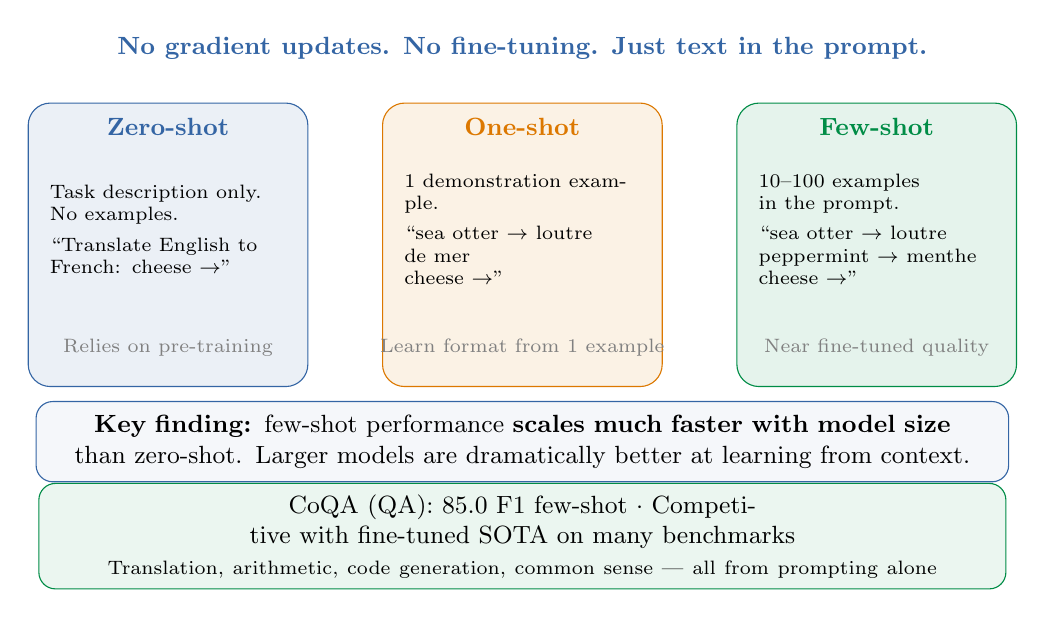
\begin{tikzpicture}
  % Three paradigms
  \node[font=\small\bfseries, text=popblue] at (0, 3.5) {No gradient updates. No fine-tuning. Just text in the prompt.};

  % Zero-shot
  \node[draw=popblue, fill=popblue!10, rounded corners=8pt, minimum width=3.5cm, minimum height=3.6cm, text width=3.2cm, align=center, inner sep=5pt] at (-4.5, 1) {};
  \node[font=\small\bfseries, text=popblue] at (-4.5, 2.5) {Zero-shot};

  \node[font=\scriptsize, text width=3cm, align=left] at (-4.5, 1.2) {
    Task description only.\\No examples.\\[3pt]
    ``Translate English to\\French: cheese $\to$''
  };
  \node[font=\scriptsize, text=gray] at (-4.5, -0.3) {Relies on pre-training};

  % One-shot
  \node[draw=orange1, fill=orange1!10, rounded corners=8pt, minimum width=3.5cm, minimum height=3.6cm, text width=3.2cm, align=center, inner sep=5pt] at (0, 1) {};
  \node[font=\small\bfseries, text=orange1] at (0, 2.5) {One-shot};

  \node[font=\scriptsize, text width=3cm, align=left] at (0, 1.2) {
    1 demonstration example.\\[3pt]
    ``sea otter $\to$ loutre\\de mer\\cheese $\to$''
  };
  \node[font=\scriptsize, text=gray] at (0, -0.3) {Learn format from 1 example};

  % Few-shot
  \node[draw=paramgreen, fill=paramgreen!10, rounded corners=8pt, minimum width=3.5cm, minimum height=3.6cm, text width=3.2cm, align=center, inner sep=5pt] at (4.5, 1) {};
  \node[font=\small\bfseries, text=paramgreen] at (4.5, 2.5) {Few-shot};

  \node[font=\scriptsize, text width=3cm, align=left] at (4.5, 1.2) {
    10--100 examples\\in the prompt.\\[3pt]
    ``sea otter $\to$ loutre\\peppermint $\to$ menthe\\cheese $\to$''
  };
  \node[font=\scriptsize, text=gray] at (4.5, -0.3) {Near fine-tuned quality};

  % Key finding
  \node[draw=popblue, fill=popblue!5, rounded corners=6pt, text width=12cm, align=center, inner sep=5pt, font=\small] at (0, -1.5) {
    \textbf{Key finding:} few-shot performance \textbf{scales much faster with model size}\\
    than zero-shot. Larger models are dramatically better at learning from context.
  };

  % Results
  \node[draw=paramgreen, fill=paramgreen!8, rounded corners=6pt, text width=12cm, align=center, inner sep=4pt, font=\small] at (0, -2.7) {
    CoQA (QA): 85.0 F1 few-shot $\cdot$ Competitive with fine-tuned SOTA on many benchmarks\\
    {\scriptsize Translation, arithmetic, code generation, common sense --- all from prompting alone}
  };
\end{tikzpicture}
\end{center}
\end{frame}

% ============================================================
% GPT-3: FEW-SHOT SCALING
% ============================================================
\begin{frame}
\frametitle{GPT-3 --- few-shot scales with model size}

\begin{center}
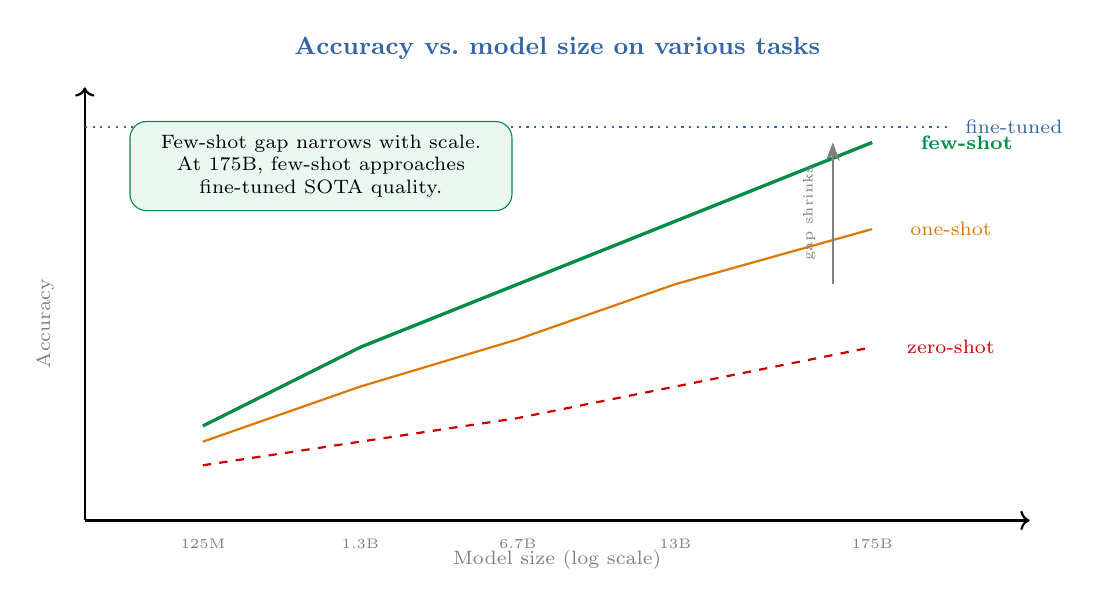
\begin{tikzpicture}
  \node[font=\small\bfseries, text=popblue] at (0, 3.5) {Accuracy vs.\ model size on various tasks};

  % Y axis
  \draw[thick, ->] (-6, -2.5) -- (-6, 3);
  \node[font=\scriptsize, text=gray, rotate=90] at (-6.5, 0) {Accuracy};

  % X axis
  \draw[thick, ->] (-6, -2.5) -- (6, -2.5);
  \node[font=\scriptsize, text=gray] at (0, -3) {Model size (log scale)};

  % X labels
  \node[font=\tiny, text=gray] at (-4.5, -2.8) {125M};
  \node[font=\tiny, text=gray] at (-2.5, -2.8) {1.3B};
  \node[font=\tiny, text=gray] at (-0.5, -2.8) {6.7B};
  \node[font=\tiny, text=gray] at (1.5, -2.8) {13B};
  \node[font=\tiny, text=gray] at (4, -2.8) {175B};

  % Zero-shot line (gentle slope)
  \draw[thick, sampred, dashed] (-4.5, -1.8) -- (-2.5, -1.5) -- (-0.5, -1.2) -- (1.5, -0.8) -- (4, -0.3);
  \node[font=\scriptsize, text=sampred] at (5, -0.3) {zero-shot};

  % One-shot line (moderate slope)
  \draw[thick, orange1] (-4.5, -1.5) -- (-2.5, -0.8) -- (-0.5, -0.2) -- (1.5, 0.5) -- (4, 1.2);
  \node[font=\scriptsize, text=orange1] at (5, 1.2) {one-shot};

  % Few-shot line (steep slope)
  \draw[very thick, paramgreen] (-4.5, -1.3) -- (-2.5, -0.3) -- (-0.5, 0.5) -- (1.5, 1.3) -- (4, 2.3);
  \node[font=\scriptsize\bfseries, text=paramgreen] at (5.2, 2.3) {few-shot};

  % Fine-tuned SOTA line (horizontal reference)
  \draw[thick, popblue, dotted] (-6, 2.5) -- (5, 2.5);
  \node[font=\scriptsize, text=popblue] at (5.8, 2.5) {fine-tuned};

  % Annotation
  \node[draw=paramgreen, fill=paramgreen!8, rounded corners=6pt, text width=4.5cm, align=center, inner sep=5pt, font=\scriptsize] at (-3, 2) {
    Few-shot gap narrows with scale.\\At 175B, few-shot approaches\\fine-tuned SOTA quality.
  };

  % Arrow showing the gap closing
  \draw[-Stealth, thick, gray] (3.5, 0.5) -- (3.5, 2.3);
  \node[font=\tiny, text=gray, rotate=90] at (3.2, 1.4) {gap shrinks};
\end{tikzpicture}
\end{center}
\end{frame}

% ============================================================
% THE EVOLUTION
% ============================================================
\begin{frame}
\frametitle{The evolution: from fine-tuning to prompting}

\begin{center}
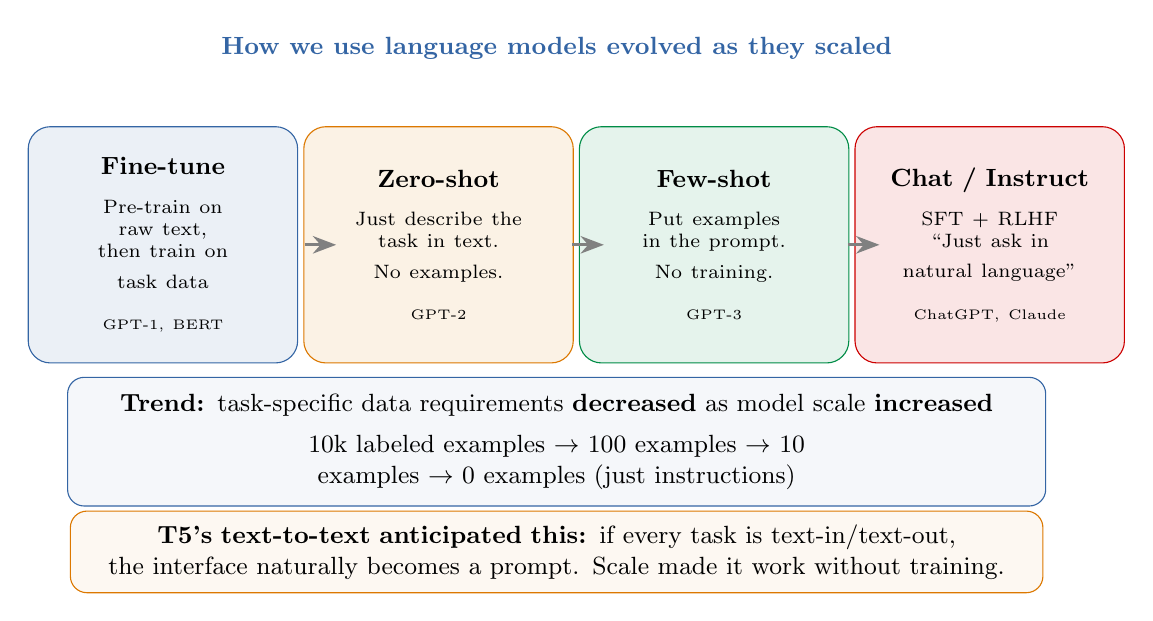
\begin{tikzpicture}
  % Timeline
  \node[font=\small\bfseries, text=popblue] at (0, 3.5) {How we use language models evolved as they scaled};

  % Stage 1: Fine-tune
  \node[draw=popblue, fill=popblue!10, rounded corners=8pt, text width=3cm, minimum height=3cm, align=center, inner sep=6pt, font=\small] at (-5, 1) {
    \textbf{Fine-tune}\\[6pt]
    {\scriptsize Pre-train on\\raw text,\\then train on\\task data}\\[4pt]
    {\tiny GPT-1, BERT}
  };

  % Stage 2: Zero-shot
  \node[draw=orange1, fill=orange1!10, rounded corners=8pt, text width=3cm, minimum height=3cm, align=center, inner sep=6pt, font=\small] at (-1.5, 1) {
    \textbf{Zero-shot}\\[6pt]
    {\scriptsize Just describe the\\task in text.\\No examples.}\\[4pt]
    {\tiny GPT-2}
  };

  % Stage 3: Few-shot
  \node[draw=paramgreen, fill=paramgreen!10, rounded corners=8pt, text width=3cm, minimum height=3cm, align=center, inner sep=6pt, font=\small] at (2, 1) {
    \textbf{Few-shot}\\[6pt]
    {\scriptsize Put examples\\in the prompt.\\No training.}\\[4pt]
    {\tiny GPT-3}
  };

  % Stage 4: Instruction
  \node[draw=sampred, fill=sampred!10, rounded corners=8pt, text width=3cm, minimum height=3cm, align=center, inner sep=6pt, font=\small] at (5.5, 1) {
    \textbf{Chat / Instruct}\\[6pt]
    {\scriptsize SFT + RLHF\\``Just ask in\\natural language''}\\[4pt]
    {\tiny ChatGPT, Claude}
  };

  % Arrows
  \draw[-Stealth, very thick, gray] (-3.2, 1) -- (-2.8, 1);
  \draw[-Stealth, very thick, gray] (0.2, 1) -- (0.6, 1);
  \draw[-Stealth, very thick, gray] (3.7, 1) -- (4.1, 1);

  % Data requirements decreasing
  \node[draw=popblue, fill=popblue!5, rounded corners=6pt, text width=12cm, align=center, inner sep=6pt, font=\small] at (0, -1.5) {
    \textbf{Trend:} task-specific data requirements \textbf{decreased} as model scale \textbf{increased}\\[4pt]
    {\small 10k labeled examples $\to$ 100 examples $\to$ 10 examples $\to$ 0 examples (just instructions)}
  };

  % Key insight
  \node[draw=orange1, fill=orange1!5, rounded corners=6pt, text width=12cm, align=center, inner sep=5pt, font=\small] at (0, -2.9) {
    \textbf{T5's text-to-text anticipated this:} if every task is text-in/text-out,\\
    the interface naturally becomes a prompt. Scale made it work without training.
  };
\end{tikzpicture}
\end{center}
\end{frame}

% ============================================================
% DATA MATTERS
% ============================================================
\begin{frame}
\frametitle{Data matters: the data scaling story}

\vspace{-0.2cm}
\begin{center}
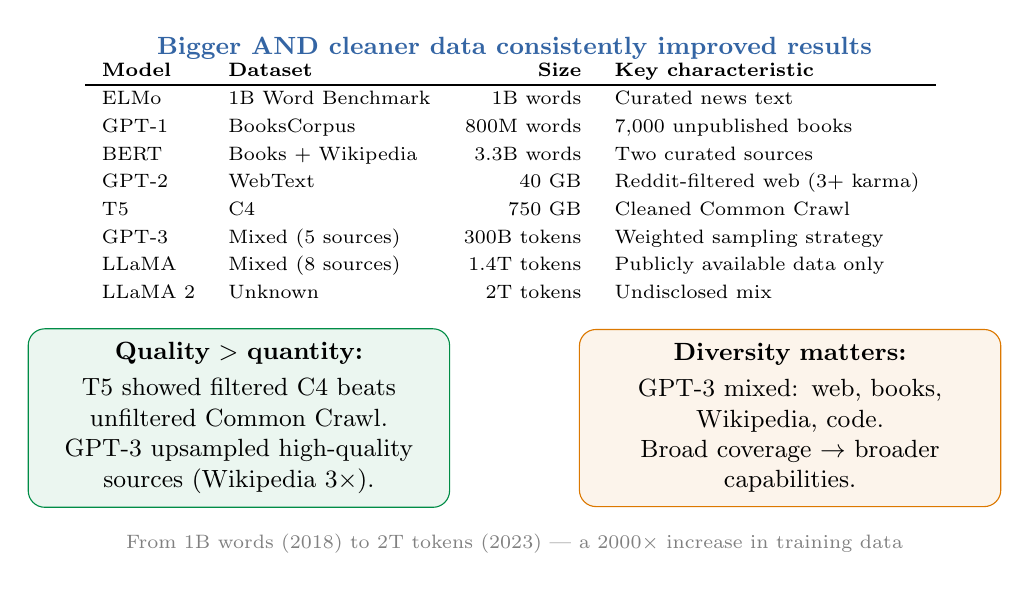
\begin{tikzpicture}
  \node[font=\small\bfseries, text=popblue] at (0, 3.2) {Bigger AND cleaner data consistently improved results};

  % Data timeline
  \renewcommand{\arraystretch}{1.25}
  \node at (0, 1.5) {
    {\scriptsize
    \begin{tabular}{l l r l}
      \textbf{Model} & \textbf{Dataset} & \textbf{Size} & \textbf{Key characteristic} \\
      \hline
      ELMo & 1B Word Benchmark & 1B words & Curated news text \\
      GPT-1 & BooksCorpus & 800M words & 7,000 unpublished books \\
      BERT & Books + Wikipedia & 3.3B words & Two curated sources \\
      GPT-2 & WebText & 40 GB & Reddit-filtered web (3+ karma) \\
      T5 & C4 & 750 GB & Cleaned Common Crawl \\
      GPT-3 & Mixed (5 sources) & 300B tokens & Weighted sampling strategy \\
      LLaMA & Mixed (8 sources) & 1.4T tokens & Publicly available data only \\
      LLaMA 2 & Unknown & 2T tokens & Undisclosed mix \\
    \end{tabular}
    }
  };

  % Key lessons
  \node[draw=paramgreen, fill=paramgreen!8, rounded corners=6pt, text width=5cm, align=center, inner sep=5pt, font=\small] at (-3.5, -1.5) {
    \textbf{Quality $>$ quantity:}\\[2pt]
    T5 showed filtered C4 beats\\unfiltered Common Crawl.\\GPT-3 upsampled high-quality\\sources (Wikipedia 3$\times$).
  };

  \node[draw=orange1, fill=orange1!8, rounded corners=6pt, text width=5cm, align=center, inner sep=5pt, font=\small] at (3.5, -1.5) {
    \textbf{Diversity matters:}\\[2pt]
    GPT-3 mixed: web, books,\\Wikipedia, code.\\Broad coverage $\to$ broader\\capabilities.
  };

  \node[font=\scriptsize, text=gray] at (0, -3.1) {
    From 1B words (2018) to 2T tokens (2023) --- a 2000$\times$ increase in training data
  };
\end{tikzpicture}
\end{center}
\end{frame}

% ============================================================
% SUMMARY TABLE
% ============================================================
\begin{frame}
\frametitle{Summary: what each model taught us}

\vspace{-0.2cm}
\renewcommand{\arraystretch}{1.35}
\begin{center}
{\scriptsize
\begin{tabular}{>{\bfseries}l c c c l}
  \textbf{Model} & \textbf{Year} & \textbf{Architecture} & \textbf{Params} & \textbf{Key contribution} \\
  \hline
  \textcolor{violet1}{ELMo} & 2018 & biLSTM & 94M & Contextual embeddings (same word $\to$ different vectors) \\[1pt]
  \textcolor{popblue}{GPT-1} & 2018 & Decoder & 117M & Pre-train + fine-tune paradigm \\[1pt]
  \textcolor{paramgreen}{BERT} & 2018 & Encoder & 340M & Bidirectional (MLM), SOTA on 11 tasks \\[1pt]
  \textcolor{orange1}{GPT-2} & 2019 & Decoder & 1.5B & Zero-shot emerges from scale \\[1pt]
  \textcolor{sampred}{T5} & 2019 & Enc-Dec & 11B & Text-to-text unification, systematic study \\[1pt]
  \textcolor{warnred}{GPT-3} & 2020 & Decoder & 175B & Few-shot in-context learning, API launch \\
  \hline
\end{tabular}
}
\end{center}

\vspace{0.1cm}
\begin{center}
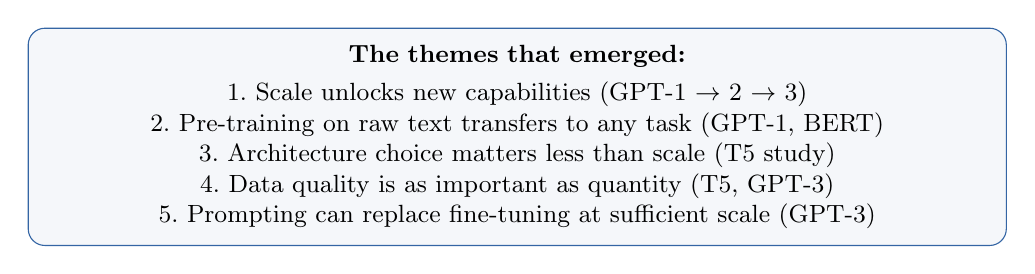
\begin{tikzpicture}
  \node[draw=popblue, fill=popblue!5, rounded corners=6pt, text width=12cm, align=center, inner sep=6pt, font=\small] at (0, 0) {
    \textbf{The themes that emerged:}\\[3pt]
    1.\ Scale unlocks new capabilities (GPT-1 $\to$ 2 $\to$ 3)\\
    2.\ Pre-training on raw text transfers to any task (GPT-1, BERT)\\
    3.\ Architecture choice matters less than scale (T5 study)\\
    4.\ Data quality is as important as quantity (T5, GPT-3)\\
    5.\ Prompting can replace fine-tuning at sufficient scale (GPT-3)
  };
\end{tikzpicture}
\end{center}
\end{frame}

% ============================================================
% QUESTIONS
% ============================================================
\begin{frame}
\begin{center}
\vspace{2cm}
{\Huge \textcolor{popblue}{Questions?}}

\vspace{1cm}
{\large Next: Prompting --- Zero-shot, Few-shot, Chain-of-Thought}
\end{center}
\end{frame}

\end{document}
